%! Tex program = xelatex
\documentclass[UTF8]{article}
\usepackage{indentfirst}
\usepackage{graphicx}
\usepackage{amsmath}
\usepackage{float}
\usepackage{listings}

\title{Discrete Mathematics}
\author{Zhengren Wang 2019081308021}
\date{05/28/2020 Thu }
\begin{document}
\maketitle

\part{9.6}
\begin{description}
    \item[3]Is $(S, R)$ a poset if $S$ is the set of all people in the world and $(a, b)\in R$, where $a$ and $b$ are people, if  \\
            a) a is taller than b             \\
            b) a is not taller than b         \\
            c) a = b or a is an ancestor of b \\
            d) a and b have a common friend   \\
            
            a) No          \\
            b) Yes         \\
            c) Yes         \\
            d) No          \\
            

    \item[23]Draw the Hasse diagram for divisibility on the set  \\

            a) {1, 2, 3, 4, 5, 6, 7, 8}.    \\
            b) {1, 2, 3, 5, 7, 11, 13}.     \\
            c) {1, 2, 3, 6, 12, 24, 36, 48} \\

            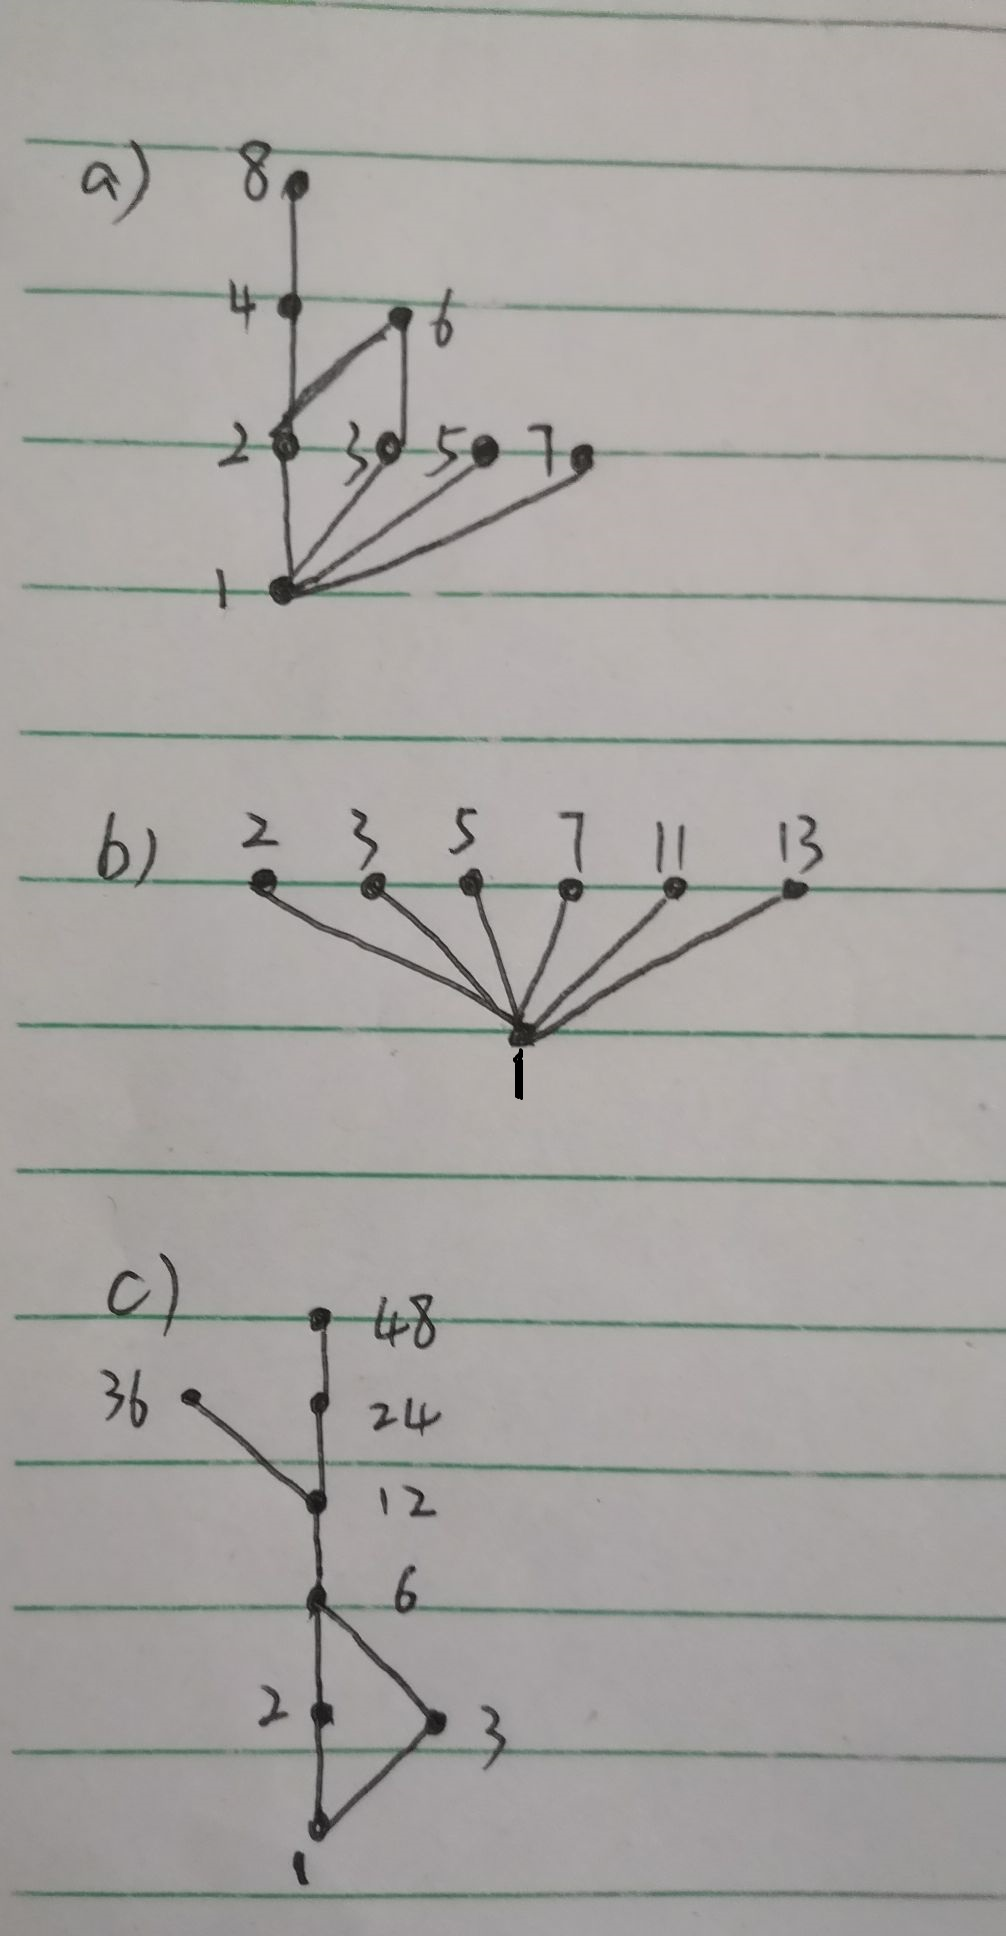
\includegraphics[scale=0.2]{../imgs/hasse.jpg}




\end{description}

\end{document}
